As we are physisicts, in this section we will start by introducing fundamental biological concepts, before specializing in the fruit fly. \\
We we will go through a short, broad explanation of the amount of information that is kept on cell- and embryo-level. We will then talk about the fascinating biology allows each cell to YYY the creation of a [living animal]. Finally we will use all these newly learned concepts to introduce the model we will be working with. By the end, we hope for the addition of every term and parameter in the model to seem sensible and biologically justified. \todo{rephrase}


\section{Broken Symmetries and Genetic Patterning}
% \section{Everything}
\label{sec:theory-polarity}
\subsection{Broken Symmetries}

Almost all animals have the same origin. Starting as a single fertilized cell, through cell-division it builds up an isotropic sphere of cells. Then, suddenly this ball will [motions] begin developing the organism to come. As animals are not spherically symmetric [citation needed], a number of symmetries need to be broken. 

In Drosophila Melongaster, after the first rounds of mitosis, the cells migrate to line the inside of the egg. This allows each of their surfaces to form distinct "outside" and "inside" domains. Through preferential adhesion\footnote{explain preferential adhesion} based on their individual surface orientation, the cells can maintain the shell structure even after removal of the surrounding shell. This gives rise to the well defined embryo-scale Inside-Outside polarity. In biology this is known as \textbf{Apical-Basal polarity} and universally seen in almost every multicellular system. 

Now, the fruit fly differs from humans zygotes, as its egg is oblong. This allows for the up/down-symmetry (Dorsal-Ventral) to be have been broken from birth. \reph 

Finally, we need some way of getting every cell to know an in-plane "forward" and "backward" direction. This polarity is called \textbf{Planar-Cell Polarity} (for obvious reasons) and is almost as ubiquitous as the Apical-Basal polarity. The way  \textit{PCP} is defined in drosophila is through a striped pattern of morphogens YY a clearly defined (nematic) direction of high gradient.

The way these pattern emerge are fascinating! 



\subsection{Genetic Patterning}
\label{sec:gen_patterns}
For a multicellular organism to go from a homogeneous cell sheet to forming their complex body plans, some organizing is needed. This complicated interplay between cells necessitates both large-scale and cell-scale control. For humans and fruit fly alike, this is done via genetic patterning.\cite{veraksa2000developmental}

As predicted by Turing, patterning is a result of "smartly"\footnote{Nature abhors a vacuous anthropomorphization} designed interactions where different chemicals assist or inhibit the production or expression of each other. 

% Now, to shake it up, \textit{Twist} \& \textit{Snail}, which might remind you of the beetles,\footnote{The species \textit{Tribozium} for example\cite{sommer1994expression}} are vital for the early development of a surviving fruit fly.

A selection of some of the most important morphogens can be seen in Table \ref{tab:morphogens} in the Appendix, and in Figure \ref{fig:MorphogenMap} their concentrations can be seen as mapped onto our virtual blastoderm.


\noindent

\begin{figure}[H]
    \centering
    \makebox[\linewidth]{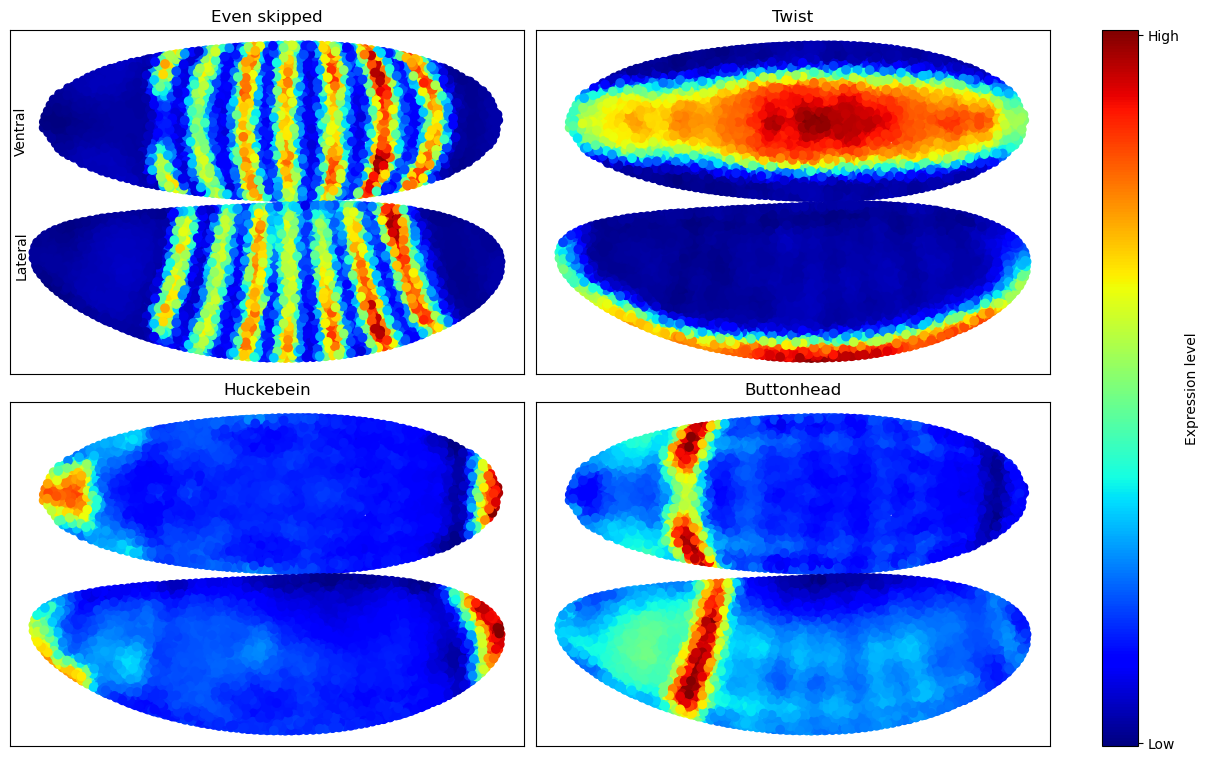
\includegraphics[width=1.2\linewidth]{chapters/Theory/figures/patterning.png}}
    \caption{The spacial distribution of a small subset of morphogens as sampled by individual cell in the Drosophila embryo. A clear attest to the remarkable and stable pattern formation Turing predicted chemicals gradients capable of producing.}
    \label{fig:MorphogenMap}
\end{figure}


Now, these concentration gradients are precise and robust enough to be picked up by the individual cells. This allows for independent differentiation on a cell-by-cell basis.\\


But for macro scale morphology changes to occur, having off-equilibrium protein concentrations are not enough; intentional changes(?) must occur. Luckily, the interaction between morphogens and mechanical deformations go both ways. It has been shown (J. Schauser et al, 2025) that a mechanical stimulus can trigger a chemical signal, thereby reinducing patterning in a feedback loop. This is called \textbf{mechanotransduction} and is believed to be vital in (for example) stable PCP-orientation. [citation needed] This means, that when cells move according to some defined polarity, they can move the signal and break other cells' symmetries along the way. \reph 


Let us take a small step back and think how extraordinary this all is. Every individual action is transcribed from the same string of DNA, where nothing happens except building one of 20-ish amino acids to form proteins. These proteins can then either help or delay the transcription of parts of (the same) DNA string.\footnote{I'm just going to say it: The \textit{Central dogma of molecular biology} is a simplification beyond the point of usefulness} It is simply the order in which these proteins are created that, together with the purely physical self-interaction, allows for infinitely convoluted stem cell to emerge.


But now, the same thing happens on the next level: Individual cells will be making simple self-alterations. The interplay between these can somehow arrive at a cohesive bigger picture. To understand this behaviour, we will look at the individual mechanical mechanisms:

\section{How Cells Move}

Most of the global large-scale cell migration seen during development of any multicellular organisms stem from a handful of seemingly simple, albeit still not well understood, active single-cell actions.\cite{walck2014cell}\\

In most YYY, cell migration consist of chemotaxis. That is, individual cells moving in the direction of a chemical gradient.\\
What we will be looking at is fundamentally different. In embryogenesis, where cells are closely bound together in epithelial sheets, the cells are able to exert forces on \textit{each other}. As can be seen on Figure \ref{fig:mysosinMeshwork}, the cells stay interconnected using membrane tethers connecting local neighborhoods. This means every cell can change its shape relative to its bordering cells, allowing for combined motion more effecient than any single cell could achieve on their own. 
% When thinkin of cell motility, chemotaxis 

% The motion we will be looking at, are of a type that is fundamentally different from Chemotaxis, with cells reacting to a local chemical concentration but not moving along a gradient [citation needed].

% The cells internal structure is called the cytoskeleton with internal \textit{motor proteins} responsible for keeping and changing the cells shape.
\begin{figure}[H]
    \centering
    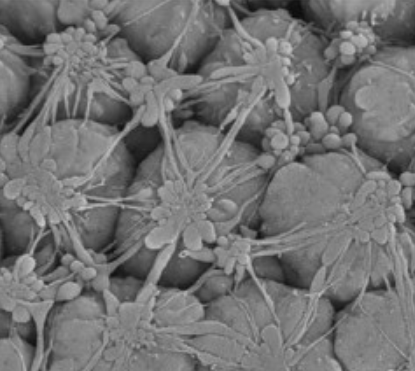
\includegraphics[width=0.6\linewidth]{chapters/Theory/figures/EM_constricting_proteins.png}
    \caption{Electron microscopy of\textit{ Myosin II} meshwork at ventral side. Taken from \citeAY{martin2010integration}}
    \label{fig:mysosinMeshwork}
\end{figure}






In Drosophila gastrulation, the exact list of 'driving effects' are surprisingly under-understood with no paper claiming certainty.\footnote{This comes down to the fact, that experiments with living cells are inherently hard} Here is a list of the fundamental single-cell active forces that is undeniably happening:

\textbf{Convergent Extension}, \textbf{Apical Constriction} and \textbf{Cell Shape Change}.

\subsection{Convergent Extension}
\label{sec:ConvergentExtension}
For elongating of sheets in a single direction, \textit{Convergent Extension} seems to be one of the most common proprietors of movement. It is made up of asymmetric cellular intercalations. In layman's terms: Cells squeezing in between each other, but mainly in one direction. 
In Figure  \ref{fig:cellIntercolation} a schematic of how cell intercalation can lead to extension can be seen.
\begin{figure}[H]
    \centering
    \begin{subfigure}{0.45\linewidth}
        \centering
    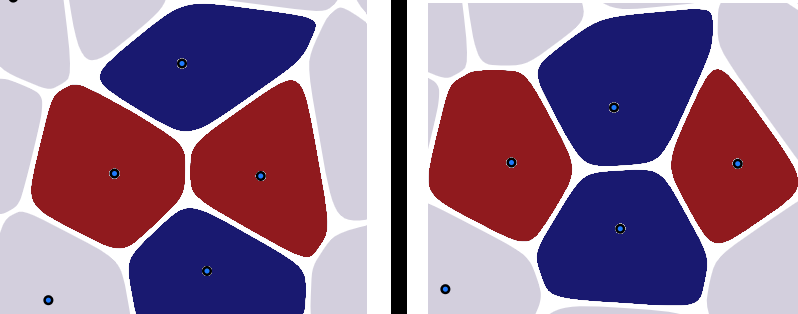
\includegraphics[width=\linewidth]{chapters/Theory/figures/ConvergentExtensionDiagram.png}
    \caption{A diagram showing how guided intercolation of blue cells can results in horizontal elongation of the cluster}
    \label{fig:cellIntercolation}
    \end{subfigure}
        \begin{subfigure}{0.45\linewidth}
        \centering
        \caption{Dyed Germ Band tissue showing clear difference in horizontal and vertical protein expressions}
    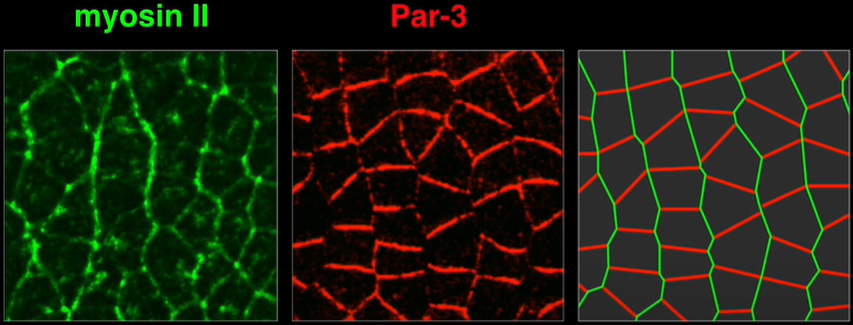
\includegraphics[width=\linewidth]{chapters/Theory/figures/bipolar-PCP.png}
    \label{fig:dyedDifferentialWall}
    \end{subfigure}
    \caption{\textbf{Left}: What is convergent extension? \textbf{Right}: \citeAY{zallen2004patterned}}
    
    \label{fig:ConvergentExtensionDiagram}
\end{figure}

The Planar-Cell polarity, as described in the previous section, can gives rise to a stark concentration-difference of different proteins between horizontal and vertical cell walls. This can be seen in Figure \ref{fig:dyedDifferentialWall}.
This means, that through anisotropically tightening of cell borders with deformations only happening in the individual cell, the full sheet scale can change shape. No cell even needs to know its position in space. 

This shrinkin of a side, leads us to the next fundamental active force.



\subsection{ Apical Constriction }
\label{sec:ApicalConstriction}
When the cell sheet wants out-of-plane bending, they turn to Apical Constriction. Apical constriction functions exactly as you would think; Myosin rings constrict the apical (outer) side of the cell, creating a smaller surface area. This leads to bending and, when enough constriction is applied, invagination. (see Figure \ref{fig:apical-constriction}). Cells has been shown the ability to constrict both isotropically and anisotropically (relative to Planar-cell Polarity).

\begin{figure}[H]
    \centering
    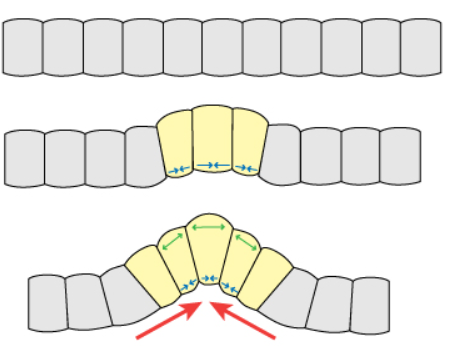
\includegraphics[width=0.3\linewidth]{chapters/Theory/figures/apical_constriction_schematic.png}
    \caption{Schematic for how apical constriction works}
    \label{fig:apical-constriction}
\end{figure}

\todo{Write a little more}
% \subsection{Cell Shape Change}
% At the onset of gastrulation, the cells are tightly packed, giving them a pronounced elongated shape. The cells can use their cytoskeleton to actively reshape their in-plane area quite drastically. [citation needed]

% \subsection{Proliferation}
% If cells are dividing in-plane, they can apply a pressure. In the stages of we are looking at, cell-division is shown to not be a driving force except in the head-region. [citation needed] As this has not been simulated in the final iteration.\\

Now, the fact that nature is thrifty with its creations, means, the few actions described above can allow for the creation of almost every type of organ in almost every type of organism. The beauty is, that understanding these fundamentals [in one system] can allow for a long list of general lessons to be learned. In this thesis we will focus on the motility required for Drosophila gastrulation to [arise]. As explained in the introduction, Drosophila is a model organism, and the fact that it has been observed for years means that it is a great onset for probing the inner workings.\todo{heavily rephrase}

Now, what is a fruit fly? 

% \section{Drosophila in Detail}
% Before we can get to the model it is necessary to introduce the star of the show. We will start out by YYY the features of the embryo before we move on to the motions it undergoes. 
% \subsection{The Drosophila Embryo in detail}
% \label{sec:drosophila-embryo-detail} 
% We will quickly outline the main morphological features of the gastrulation cycle of the embryo:
% \begin{outline}
%     \1 Posterior Midgut (PMG)
%     \1 Anterior Midgut (AMG)
%     \1 Ventral Furrow
%     \1 Dorsal Transverse Furrows
%     \1 Cephalic Furrow
%     \1 Germ Band
% \end{outline}

% \begin{figure}[H]
%     \centering
%     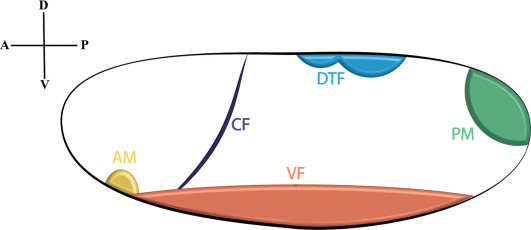
\includegraphics[width = 0.7\linewidth]{chapters/Theory/figures/morphogenic_events.jpg}
%     \caption{Summary of the morphogenetic events mapped onto the blastoderm stage embryo. Taken from \cite{gheisari2020gastrulation}. The colored parts are generally seen to be the morphogenetically active during the early part of the embryogenesis}
%     \label{fig:enter-label}
% \end{figure}

% IN OUR SIMULATION: 

% The Germ Band is defined as all cells expressing a sufficient YY of the two striped genes \textit{Eve} and \textit{Run} the at the onset of gastrulation. \cite{zallen2004patterned}


\newpage
\section{The Drosophila Gastrulation in detail}
In 1975 Bownes et al. split the development of the fruit fly from fertilised egg to hatched larvae into 17 distinct events.\cite{bownes1975photographic} We will be looking at stages 5 through 7, lasting about 15 minutes. These are characterized by having the first mesoscopic morphogenetic movements and setting the stage for all morphology to come.

When looking at the embryo, the following parts will be the most active, important and relevant to our [project:]


\begin{figure}[H]
    \centering
    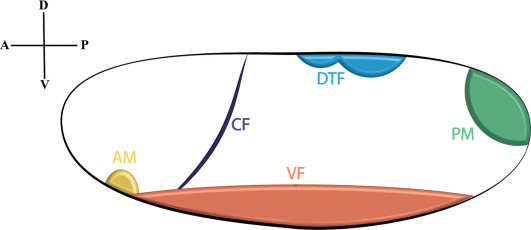
\includegraphics[width = 0.9\linewidth]{chapters/Theory/figures/morphogenic_events.jpg}
    \caption{Taken from \citeAY{gheisari2020gastrulation}. \\
    VF: Ventral Furrow\\
    PMG: Posterior Midgut\\
    CF: Cephalic Furrow\\
    Germ-band: A band of germs}
    \label{fig:enter-label}
\end{figure}


The Drosophila gastrulation consist of a series of interconnected but independently localized cell movements. We will now present an abridged overview, roughly ordered in time:





\newpage

\begin{figure}[H]
    \centering
    \vspace*{-1cm}\makebox[\textwidth]{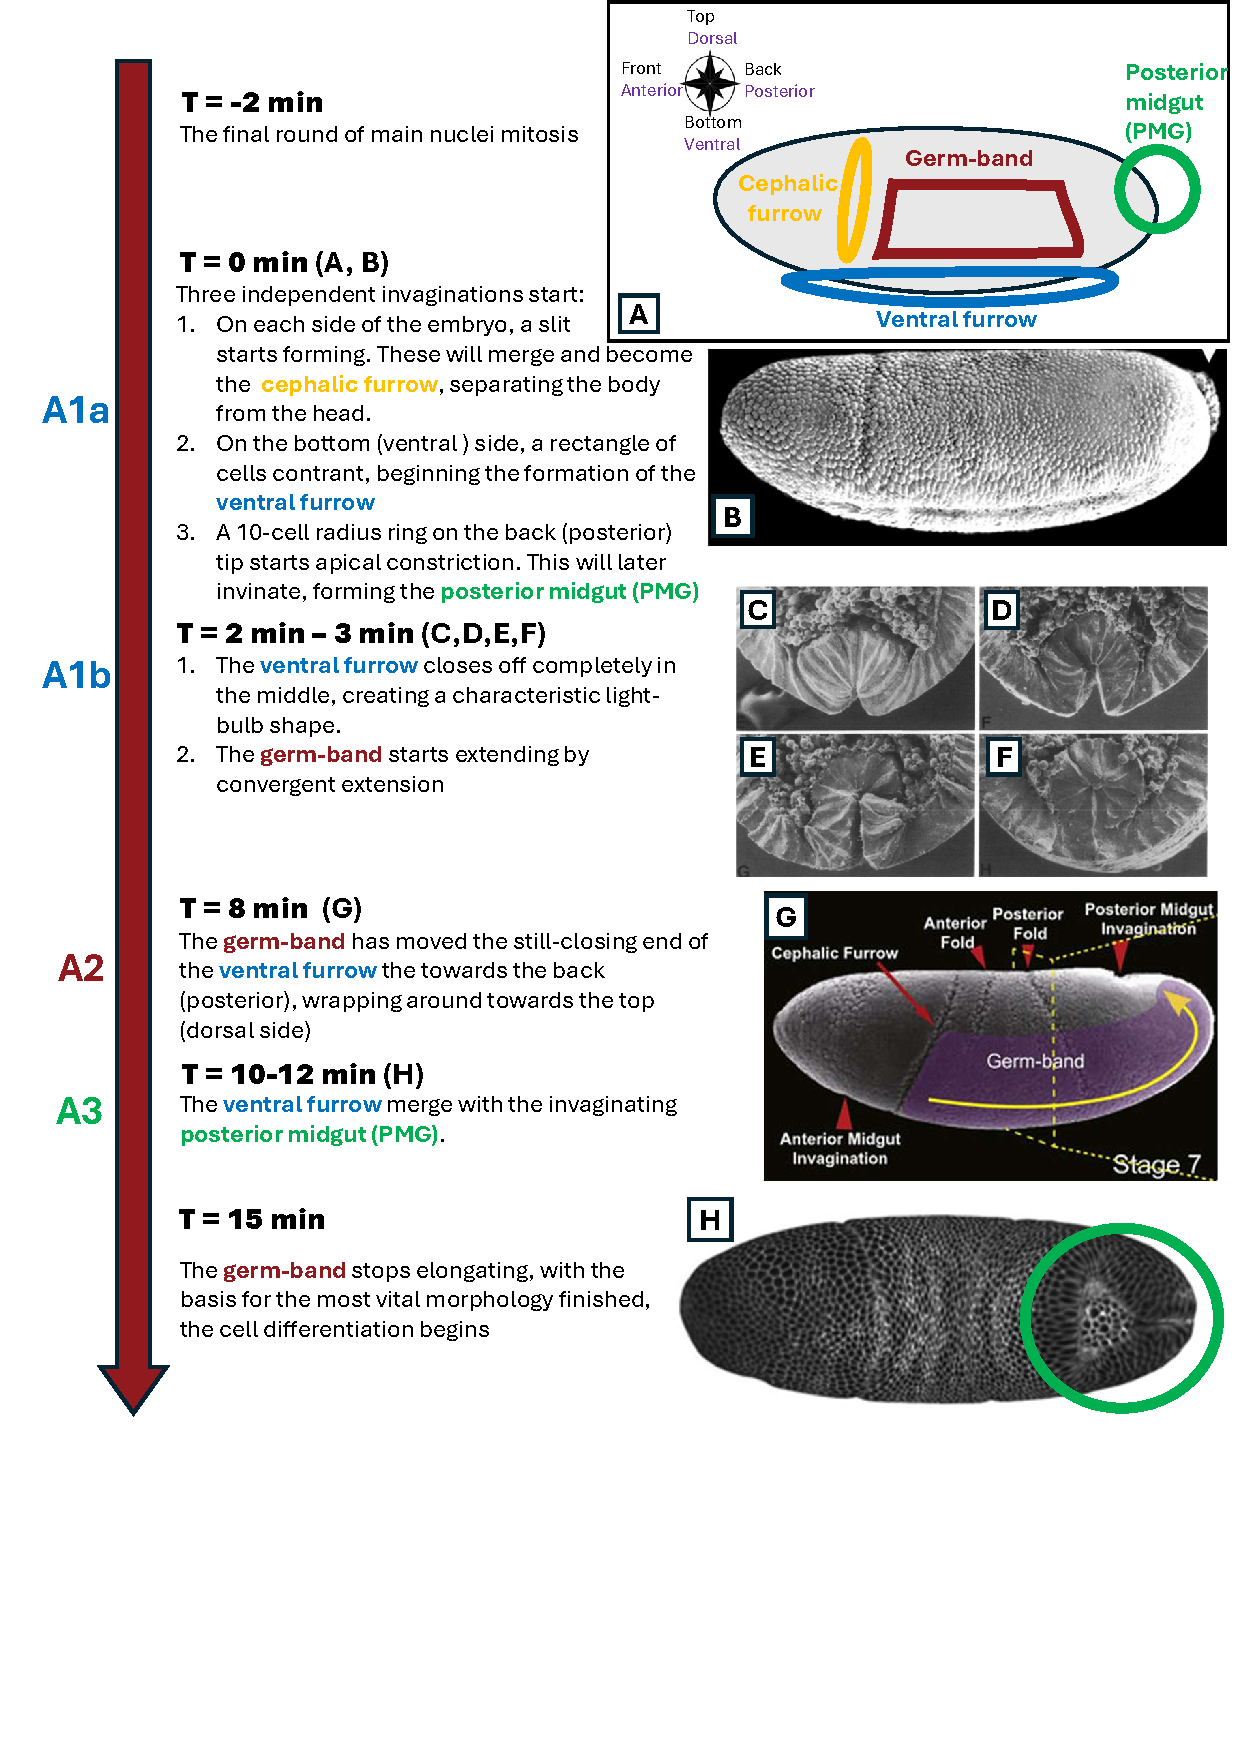
\includegraphics[width=0.8\paperwidth]{chapters/Theory/figures/Timeline_v2.pdf}}
    \caption{Caption}
    \label{fig:big-timeline}
\end{figure}
\newpage
\addtocounter{figure}{-1}
\begin{figure} [t!]
  \caption{(Previous page.) \\ A somewhat comprehensive explanations of the most important past of the initial parts of the gastrulation.
  }
\end{figure}
\vspace*{5cm} 
\textit{This page is intentionally left blank so the previous page can be taken and kept as a cheat-sheet for later referencing. }
\newpage
\section{Previous attempts at simulation}
In silico models has provided multiple working examples of all the aforementioned embryogenesis events with multiple different approaches. A lot has been learned through the comparison between model and YY, especially taking onset in Drosophila.\\
When studying the biomechanics of morphogenesis there seems to be two main strategies:\\
1) Choose a single morphogenetic event, studying in detail. (The ventral furrow formation (A2)\todo{MAKE NUMBER MATCH!!!}, for example)\\
2) Choose a single active phenomenom and look at simulating it "in a vacuum", comparing to an isolated cell-sheet.(convergent extension, for example (Section \ref{sec:ConvergentExtension})) 


The first can grant a detailed understanding of the physics/chemistry at play.

Examples of 1) are early Apical Constriction 2d cross section \cite{odell1981mechanical}, 

Focusing on pressure and tensile forces 

The second approach 
Ones who focus on a phenomenon (2)) are: 

requiring it to be done in 2d.



2d cell shape change \cite{krajnc2018fluidization}

State-of-the-art vertex based compared to other types \cite{fletcher2017mechanocellular}

The problem is, that Avogadro constant is quite large. Models that look at sub-parts of cells are often computationally heavy. When looking for off-lattice cell-center-based model, not many shows up. An example (only non-polar interactions) (a maximum of 600 cells) (from what I can see only used on C. Elegans) (assumed spherical, i.e. not inherently useful for epithelial sheets)\cite{atwell2015mechano}


It is mainly finite-element simulations have dominated the field when studying the physics of tubologenesis, tissue-folding etc.  

This allows for a , but the interplay between different parts of the embryo, different [force-types] and YYY are ignored.  



Removing the focus from the on the biomechanics of a single part, instead focusing on the YYY, Just like nature is reusing

This all leads us to the star of the show:

\section{The Model}

This section takes it onset in the model described in \citeAY{nissen2018theoretical} and later expanded in \citeAY{nielsen2020model}. Whenever we deviate from the existing literature, this will be stated clearly.\\

As we know global-scale changes in physical structure during gastrulation all arise from single cell actions with little discernible individual movement. The model is built around simply simulating the movement of the center of mass of the cells along with their individual orientation. It is based on the following intercellular potential: \reph

\begin{equation}
    V_{ij}=e^{-r_{ij}}-A_{ij}e^{-r_{ij}/\beta}
\end{equation}

Where $r_{ij}$ is the distance between two cells $A_{ij}$ is a attraction factor what will be explained later, and $\beta$ is a constant (usually 5, which is very constant). 

Where the individual cell wants to minimize the quantity 
\begin{equation}
    U_i = \sum_j V_{ij}
    \label{eq:totalPot}
\end{equation}
Here the sum over $j$ is over all Line of sight/Voronoi neighbors, which should remind you of the nearest neighbor protein connections in Figure \ref{fig:mysosinMeshwork}. 


For $A_{ij}=1$ (we will soon expand on this term), the potential can be seen in Figure \ref{fig:potential}.
\begin{figure}[H]
    \centering
    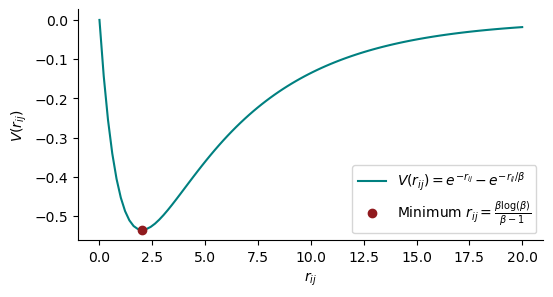
\includegraphics[width=1.\linewidth]{chapters/Theory/figures/potential.png}
    \caption{The potential well our point particles lie in, with the minimum (i.e. effective cell size) drawn in. Here we also see the role of $\beta$ as responsible for regulating the relaxation-distance}
    \label{fig:potential}
\end{figure}

The shape of the potential well should remind you of the Yukawa/ Lennard-Jones potential, which also rely on strong short-range repulsion and weaker, longer-ranged attraction.

$\cdots$\\
Now, just like nature, we will want to break some symmetries to allow for interesting morphologies to emerge.\\
The principal idea is to elevate the Apical-Basal and Planar-Cell polarities (as described in previous sections) by seeing them as explicitly stated polarization vectors with rules for self- and neighbor interaction.
Introducing a more complicated $A_{ij}$-parameter we see it as a sum of four terms
\begin{equation}
    A_{ij}=\sum_{n=0}^{3}\lambda_n  S_n
\end{equation}

As these $S_n$ are come with a negative sign they are the attractive terms.
Lets one by one.

We would want a simple term that allows for non-polar attraction between cells. We start out by: 
\begin{equation*}
    S_0 = 1
\end{equation*}

Running this, we would have a simulation with all cells forming a sphere. Much like the earliest stage of the drosophila embryo.

The first symmetry that is broken is the inside-outside symmetry. Introducing the (normalized) $\hat{p}$ vector for each cell allows for the \textit{Apical-Basal} polarity to be .
As previously mentioned the interplay between cell-polarisation and physical orientation goes both ways (the mechanotransduction as described in section \ref{sec:theory-polarity}). This motivates the following four terms which I will explain after introducing:

\begin{equation*}
    S_1=\left(\hat{p}_i \times \hat{r}_{i j}\right) \cdot\left(\hat{p}_j \times \hat{r}_{i j}\right)
\end{equation*}


As can be seen, the dot-product of cross products are used multiple times. This configuration can be understood for $\left(a \times b\right) \cdot\left(c \times d\right)$ as "keep a and c, and b and d respectively parallel, while keeping a and b, and c and d internally perpendicular". \todo{rephrase or cut} 

\begin{figure}[H]
    \centering
    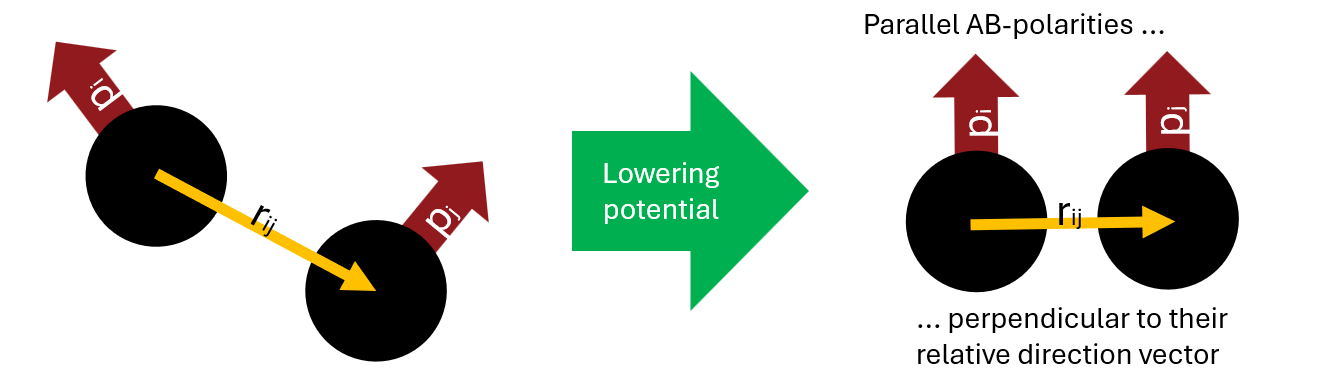
\includegraphics[width=0.3\linewidth]{chapters/Theory/figures/explainS1.png}
    \caption{A visual help for understanding the influence of the $S_1$-term (Equation \ref{eq:s1}). The orange arrow is the AB-polarity and the blue circles representations of the positions of the cells.}
    \label{fig:explain-S1}
\end{figure}

Adding the $S_1$-term to our potential we will begin seeing sheets of cells. Placing them inside an egg and letting them migrate towards the shell, we would see the second stage of uniformly distributed cells lining the inside of the egg. \\

We will now need to break some in-plane symmetry to get the \textit{Planar-Cell}-polarity:
\begin{equation*}
    S_2=\left(\hat{p}_i \times \hat{q}_{i}\right) \cdot\left(\hat{p}_j \times \hat{q}_{j}\right)
\end{equation*}
This term keeps the Apical-Basal and Planar-Cell-polarities perpendicular within each cell, but aligned across cells. This gives a stable and consistent, but changeable in-plane orientation vector for each cell. We now have a possible direction of motion.\\

To use this, we will take inspiration from the Convergent Extension (Section \ref{sec:ConvergentExtension}) and introduce 

\begin{equation*}
    S_3=\left(\hat{q}_i \times \hat{r}_{i j}\right) \cdot\left(\hat{q}_j \times \hat{r}_{i j}\right)
\end{equation*}

This term is lowest when the Planar-Cell-polarities are aligned but perpendicular to eachs NB-direction-vector \todo{find a good word for this}. In the realm where this term dominates, the cell sheets created by $S_1$ are exchanged for lines of cells perpendicular to their PCP-vectors. 
\todo{make figure}


The full array is therefore:

\begin{subequations}
\begin{align}
S_0&=1\label{eq:s0}\\
S_1&=\left(\hat{p}_i \times \hat{r}_{i j}\right) \cdot\left(\hat{p}_j \times \hat{r}_{i j}\right)\label{eq:s1}\\
S_2&=\left(\hat{p}_i \times \hat{q}_{i}\right) \cdot\left(\hat{p}_j \times \hat{q}_{j}\right)\label{eq:s2}\\
S_3&=\left(\hat{q}_i \times \hat{r}_{i j}\right) \cdot\left(\hat{q}_j \times \hat{r}_{i j}\right)\label{eq:s3}
\end{align}
\end{subequations}

If the constraint $\sum_{n=1}^{3}\lambda_n=1$ is not fulfilled, the effective cell size is not constant.\\

\textbf{important} the $\hat{p}_i$'s and $\hat{q}_i$'s are normalized each frame.




$S_3$ allows for convergent extension, Now, we would like to emulate apical constriction (Section \ref{sec:ApicalConstriction}) this is done via \textbf{Wedging}\\




As apical constriction is the single cells way of creating larger-scake furrows and wedges, we implement this by changing the $\hat{p}_i$'s to 'trick' each cell into believing their neighbors are differently oriented (thereby changing the relaxation angle):

\begin{equation}
    \tilde{{p}}_i = \frac{\hat{p}_i-\alpha \widehat{{r}}_{i j}}{|\hat{p}_i-\alpha \widehat{{r}}_{i j}|} 
\end{equation}
(A similar expression can be made for anisotropic wedging, taking  $\hat{q}_i$'s into account.)

Now, diverging from the original ideas, we [morph] the basic model into something that is useful in for our specific usecase.

Now all cells are defined through a cell type, which simply means they have a $\lambda$-array and a $\alpha$ associated with them.
\textbf{Differential adhesion}
A slight was needed for the YYY. The interaction between the ventral furrow cells (cell type 2) and cells of other types where scaled by a factor of 5\% (multiplied by 0.95) so as to discourage unneccesary mixing. 
\textbf{better apical constriction}
To emulate the lowering of apical surface area, invaginating cells ($\alpha > 0$) got an increase in their $\lambda_1$'s (in Equation \ref{eq:s1}) making their relaxation distance shorter. This had the added benefit of echoing the tighter bonds in constricting cell clusters. [citation maybe needed]

\textbf{S1 -- S0}
When any of the invaginating YYY closed off, they S1-terms. A line of code was added, to combat this: When two apical sides interacted, they were only allowed to interact as non-polar, i.e. their S1-terms where changed into S0.


\textbf{Nematic $S_2$ and $S_3$} write this

\textbf{Patterning}
As we have about 5000 cells, this effectively gives 25000 parameters.

To combat this, we again look to nature and remember the patterning Section \ref{sec:gen_patterns}. Somehow all the information a cell needs will be in these boundary conditions.\\
Luckily for us, straight from Wikipedia:
"Some of the earliest and best-studied morphogens are transcription factors that diffuse within early Drosophila melanogaster (fruit fly) embryos."


In \cite{shinyDVEX} they map out the relative gene expression for the drosophila embryo and YYYY. We can then take YYY and project them onto our embryo. \todo{make sound harder}. Taking these  and cross referencing with 

In Section \ref{App:morphogens} in the Appendix the exact choices made and justifications can be seen.

We now set up a pipeline allowing for a simple run to go [something like this]:

\begin{lstlisting}
# Start a new egg from a relaxed base shape
GE = GeneExpression("path/to/base_shape")

# combine morpogens through [and, or, not]
twist_and_snail = GE.and_gene(GE.gene("twi"), GE.gene("sna"))

# Make a cut-off (20%) and define cells as 
#    belonging to a cell type (2) 
GE.add_expression(twist_and_snail, 0.2, 2) 

# save and run simulation
GE.save("name_of_expression_profile",)

\end{lstlisting}

\textbf{Where to put this?}
As we estimate the cells to move slowly and in a friction-filled viscous YYY (the low Reynolds-regime), each timestep the cells move as subjects to overdamped dynamics. For a cells position $r$ and the two polarization vectors, :

\begin{equation}
    \frac{d \bar{x}_i}{d t}=-\frac{d U_i}{d \bar{x}_i}+\eta \hspace{1.5cm}|\hspace{1.5cm}  \bar{x} \in \{\bar{r}, \bar{p}, \bar{q}\}
\end{equation}

where $\eta$ is uncorrelated Gaussian noise and U is the total potential as defined in Equation \ref{eq:totalPot}.

Given we choose 4 different cell types and no non-polar interaction, we have cut down to only have 16 parameters. Locking in the $\lambda$'s lowers this even further to about 6 parameters. 

Is it possible to accurate simulate the origin of life using 6 parameters? Read on to find out!

A note for reading on:\\
As the model is purely point-based, whenever we speak of inter-cellular junctions, neighbors, areas or angles, everything is inferred from the modeled point cloud and Voronoi-neighbors.

\section{Implementation}
The gradient is calculated via an automatic differentiation engine (The PyTorch-framework specifically) and the simulation time steps are calculated via Euler integration.

This is not interesting to read about, so extensive notes on the actual implementation along with pseudocode, can be found in Section \ref{App:Code} in the Appendix.

